\documentclass[dvisvgm,tikz,border=4pt]{standalone}
\usepackage{amsmath,amssymb}

\usetikzlibrary{arrows.meta,positioning,automata,shapes,shapes.misc,calc,decorations.pathmorphing,decorations.markings,angles,quotes,patterns,mindmap,matrix,knots,hobby,trees}
\tikzset{->-/.style={decoration={markings, mark=at position 0.5 with {\arrow{Stealth}}}, postaction={decorate}}}
\begin{document}
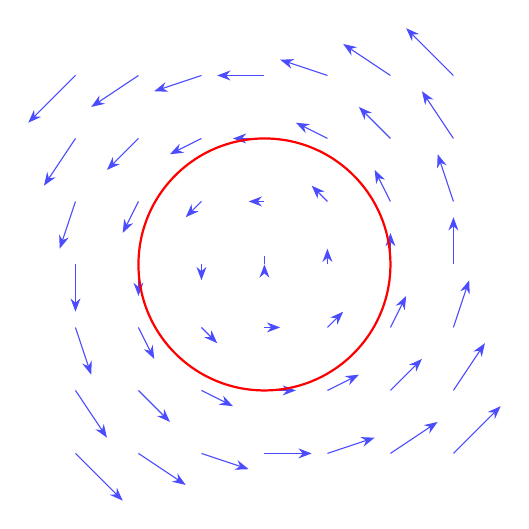
\begin{tikzpicture}[scale=0.8, >=Stealth]
\foreach \x in {-3,...,3} \foreach \y in {-3,...,3} { \draw[->, blue!70] (\x,\y) -- ++({-0.25*\y},{0.25*\x}); }
\draw[thick, red] (0,0) circle (2);
\end{tikzpicture}
\end{document}
